\section{Method}
\label{sec:method}

\vspace{-0.5em}
\subsection{Preliminaries}
\label{sec:prelim}

We consider one head of a linear attention model with a recurrent state matrix $S_t\in\mathbb{R}^{d_k\times d_v}$, query $q_t\in\mathbb{R}^{d_k}$, and value and output $v_t,o_t\in\mathbb{R}^{d_v}$.
We study recurrences whose update is a diagonal decay followed by a single rank-one delta-rule~\citep{schlag2021linear} update:
\begin{equation}
  S_t = \Diag(\alpha_t)S_{t-1}
      + k_t\bigl(v_t-S_{t-1}^{\top}\beta_t\bigr)^{\top},
  \qquad o_t=S_t^{\top}q_t.
  \label{eq:general}
\end{equation}
Here $\Diag(\alpha_t)$ is the diagonal decay~\citep{team2025kimi}, $k_t\in\mathbb{R}^{d_k}$ is the key vector, and $\beta_t\in\mathbb{R}^{d_k}$ is a read vector ($\beta_t=0$ for models without the delta rule).
Appendix~\ref{app:instances} shows how other linear attention models fit this form.

For state quantization, denote $\hat S=\quant_b(S)$, where $\quant_b$ is the $b$-bit quantization operator, $S$ is the original state, and $\hat S$ is its quantized representation, including scale metadata.
We use $S_t^{\mathrm{FP32}}$ for the independent trajectory of \eqref{eq:general} without state quantization and $E_t=\dequant_b(\hat S_t)-S_t^{\mathrm{FP32}}$ for its quantization-induced deviation, where $\dequant_b$ is the corresponding dequantization operator.
When a quantized state participates in arithmetic below, its dequantization is implicit.

\subsection{Per-window quantization}
\label{sec:round1}

A na\"ive state-quantized model quantizes and dequantizes the full state after \emph{every} decode step.
At step $t$, it first computes the full-precision updated recurrent state \hlinline{fpmark}{S_t} from the previously quantized state \hlinline{quantmark}{\hat S_{t-1}}, then quantizes the resulting new recurrent state:
\begin{equation}
  \begin{aligned}
    \hfp{S_t} &= \Diag(\alpha_t)\,\hq{\hat S_{t-1}}
       + k_t\bigl(v_t-\hat S_{t-1}^{\top}\beta_t\bigr)^{\top},\\
    \hq{\hat S_t} &= \quant_b\bigl(\hfp{S_t}\bigr).
  \end{aligned}
  \label{eq:naive}
\end{equation}
\begin{wrapfigure}[15]{r}{0.40\linewidth}
    \vspace{-1\baselineskip}
    \centering
    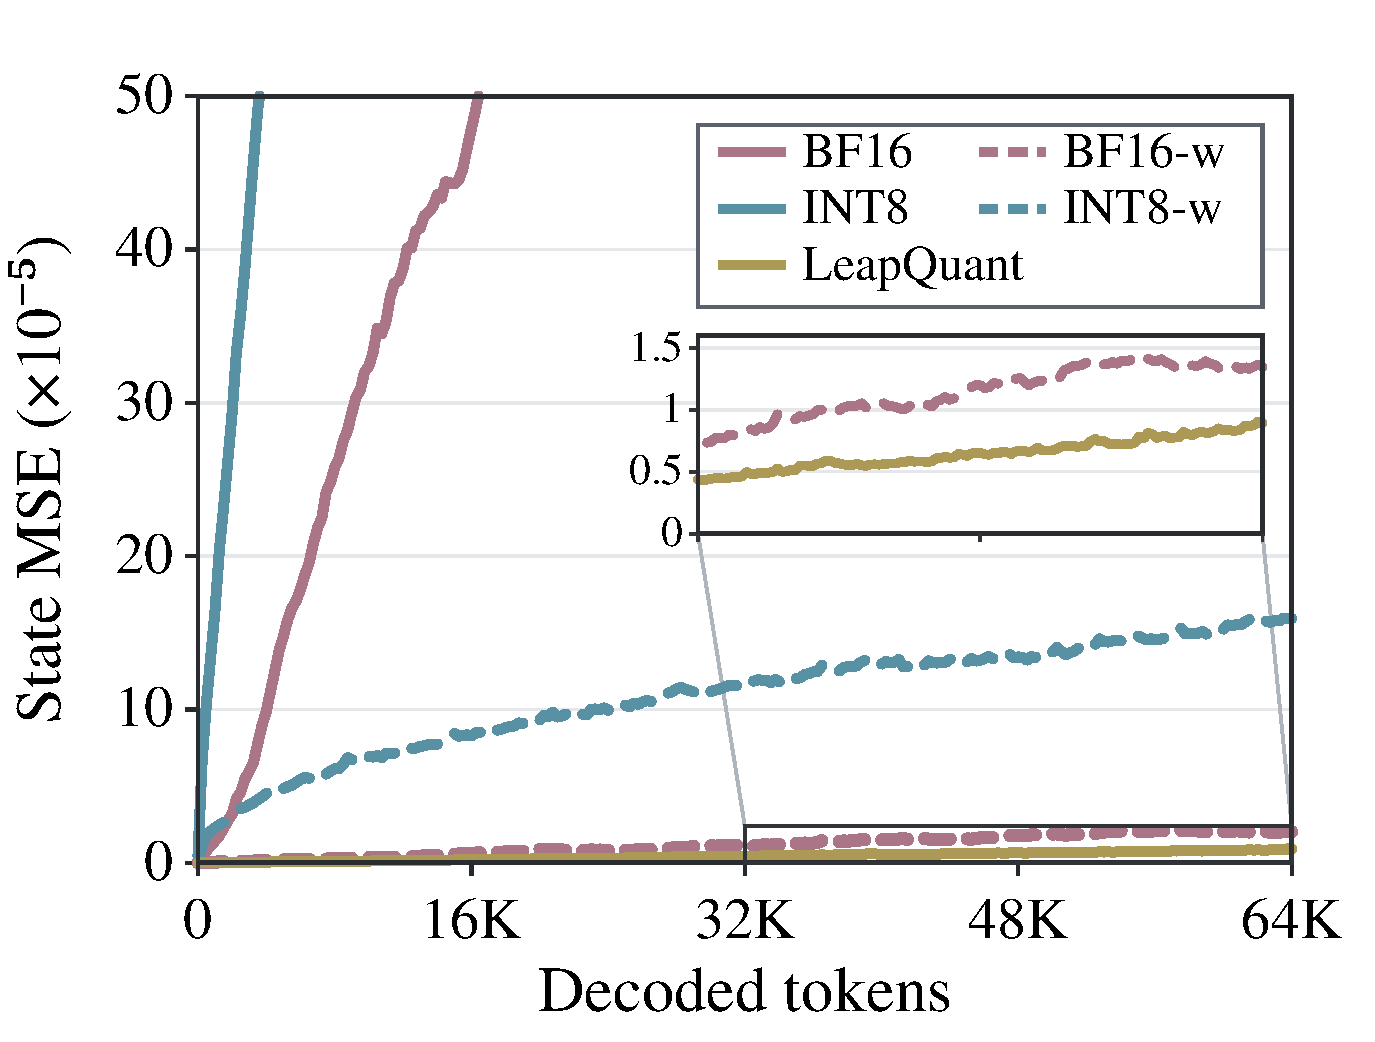
\includegraphics[width=0.95\linewidth]{figures/state-mse-paper.pdf}
    \caption{State MSE over 64K decoded tokens on PG-19 (Qwen3.5-9B); -w quantizes once per window.}
    \label{fig:state-error}
\end{wrapfigure}
%
\noindent Because every update starts from an already quantized state, its rounding error is carried into subsequent steps and can accumulate over long contexts (Appendix~\ref{app:deviation}).
Per-step quantization therefore introduces a new error at every token.
Figure~\ref{fig:state-error} tracks the error of the quantized state against the FP32 trajectory of Qwen3.5-9B over 64K decoded tokens.
Under per-step quantization, the error grows steadily with the context length, even for BF16.
Stochastic rounding helps little, as it only lowers the BF16 error at 64K by 3× and makes INT8 diverge.
In contrast, quantizing only once per 16-token window, as introduced below (the -w variants), lowers the error at 64K by $100\times$ for BF16 and by $39\times$ for INT8.
\method{} further reduces the error of each window-boundary quantization and keeps the lowest error throughout, even below per-window BF16 at half the bits.

\vspace{0.5\baselineskip}
Motivated by the error growth in Figure~\ref{fig:state-error}, we propose \textbf{per-window quantization} (Figure~\ref{fig:per-window}).
We write each update as a decay followed by a rank-one update whose correction vector $u_i$ is computed from the previous state.
For every instance of \eqref{eq:general}, this update is described by the decay $\alpha_i$, the key vector $k_i$, and the computed correction $u_i$:
\begin{equation}
  u_i=v_i-S_{i-1}^{\top}\beta_i,
  \qquad S_i=\Diag(\alpha_i)S_{i-1}+k_i u_i^{\top}.
  \label{eq:record}
\end{equation}
We now consider a sequence of $p$ consecutive tokens fed into the linear state.
For simplicity, index them as tokens $1,\ldots,p$.
We keep the quantized boundary state $\hat S_0$ fixed and buffer the $p$ tuples $(\alpha_i,k_i,u_i)$ in higher precision.
For $a\le b$, denote the cumulative decay from step $a$ through step $b$ by $\Gamma_{a:b}=\Diag(\alpha_b)\Diag(\alpha_{b-1})\cdots\Diag(\alpha_a)$, and set $\Gamma_{a:b}=I$ when $a>b$.
Then, for any $1\le\ell\le p$, unrolling \eqref{eq:record} from $\hat S_0$ yields (Appendix~\ref{app:readout})
\begin{equation}
  \begin{aligned}
    \hfp{S_\ell} &= \Gamma_{1:\ell}\,\hq{\hat S_0}
       + \sum_{j=1}^{\ell}\Gamma_{j+1:\ell}\,k_j u_j^{\top},
       \qquad 1\le\ell\le p,\\
    \hq{\hat S_p} &= \quant_b\bigl(\hfp{S_p}\bigr).
  \end{aligned}
  \label{eq:window}
\end{equation}
This is the chunk-level form that linear attention uses in training and prefill~\citep{yang2024parallelizing,yang2025gated}: intermediate states are expressed through the boundary state and the buffered tuples, so the full state is never re-quantized within the window.
Only at $\ell=p$ do we materialize $S_p$ and quantize it for the next window as $\hat S_p$.
This reduces the quantization frequency by a factor of $p$ and substantially lowers the state error over long contexts.

\begin{figure}[t]
    \centering
    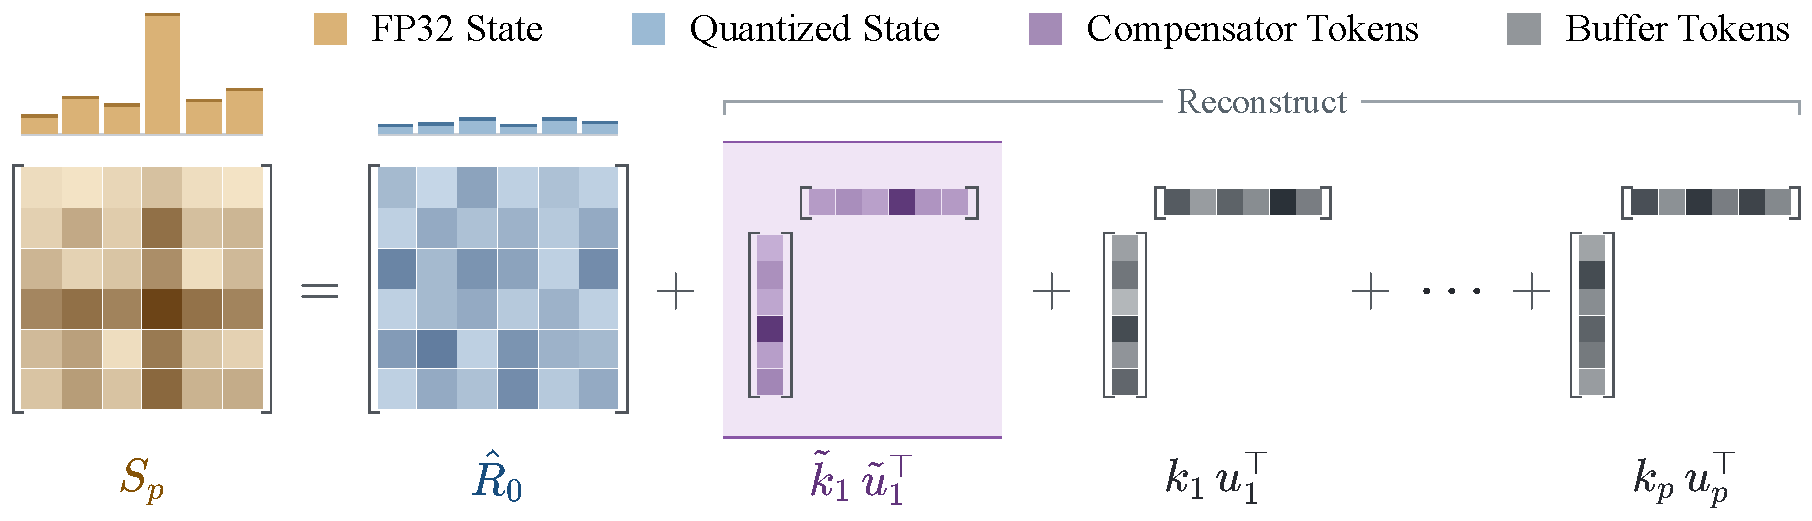
\includegraphics[width=0.9\linewidth]{figures/compensator-tokens-paper.pdf}
    \caption{Per-window state reconstruction with Compensator Tokens. The FP32 state is split into a low-bit quantized residual, a few higher-precision Compensator Tokens that capture its dominant large-magnitude structure, and the buffered real-token updates of the window. The Compensator Tokens absorb dominant outliers, flattening the residual's row $\ell_2$ norms and making it easier to quantize.}
    \vspace{-1.5em}
    \label{fig:ghost-tokens}
\end{figure}


\subsection{Compensator Tokens}
\label{sec:round2}

Although per-window quantization reduces the quantization frequency, the reconstructed state $S_p$ can contain large-magnitude outliers concentrated in a few rows and columns (Figure~\ref{fig:state-heat}(a)), and a few singular components carry most of its energy (Figure~\ref{fig:energy}).
These outliers dominate the quantization scale, forcing most entries to be represented with unnecessarily coarse quantization steps.
To address this problem, we introduce \textbf{Compensator Tokens} (Figure~\ref{fig:ghost-tokens}), which reduce outlier-induced quantization error while integrating naturally with per-window quantization.

Before quantizing $S_p$, we fit a rank-one matrix $\tilde k\tilde u^{\top}$ to capture its dominant large-magnitude structure.
We subtract this matrix from $S_p$ and quantize only the residual $R_p$.
The largest values are therefore kept out of the tensor being quantized, reducing its dynamic range and alleviating the quantization pressure:
\begin{equation}
  \begin{aligned}
    (\tilde k,\tilde u)
       &= \operatorname*{arg\,min}_{k,u}
          \bigl\lVert\hfp{S_p}-ku^{\top}\bigr\rVert_F,\\
    R_p &= \hfp{S_p}-\tilde k\tilde u^{\top},
       \qquad \hq{\hat R_p}=\quant_b(R_p),\\
    \hrec{\tilde S_p} &= \dequant_b\bigl(\hq{\hat R_p}\bigr)
       +\tilde k\tilde u^{\top}.
  \end{aligned}
  \label{eq:compensator}
\end{equation}
Here $\lVert\cdot\rVert_F$ is the Frobenius norm.
We call the pair $(\tilde k,\tilde u)$ a \textbf{Compensator Token} as it preserves the dominant state component in higher precision and, together with identity decay, has the same rank-one update form as a real token in \eqref{eq:record}.
Unlike a real input token, it is not produced by the model and does not generate an output.
It exists only in the window representation and is placed before the real-token updates of the next window.
Since the decode kernel operates directly on rank-one updates, it processes the Compensator Token through the same path as the real tokens without any model-specific modification.

At the start of the next window, the quantized residual and the compensator tokens together represent the initial state.
The decode kernel processes the compensator tokens before the real-token updates, so subsequent updates and outputs use the combined state without the need for an extra kernel.

At the end of each window, we reconstruct $S_p$ from the quantized residual, the current compensator tokens, and the window's real-token updates.
We then discard the old compensator tokens, fit a new approximation to $S_p$, and quantize the remaining residual.
The new quantized residual and compensator tokens initialize the next window.

\begin{figure}[t]
    \centering
    \begin{minipage}[t]{0.217\linewidth}
        \centering
        \vspace{0pt}
        \vspace{0.08\linewidth}
        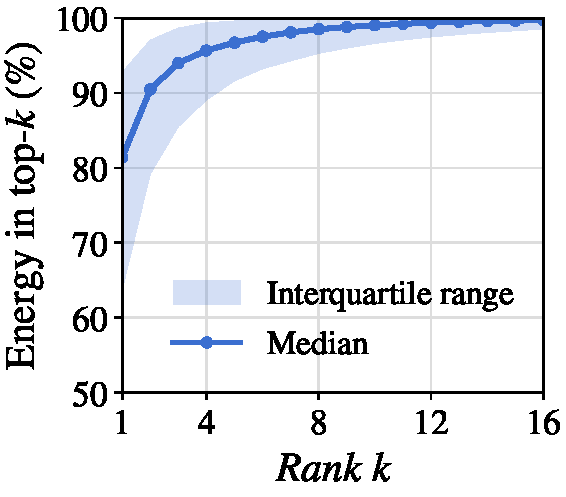
\includegraphics[width=\linewidth]{figures/state_energy.pdf}\\[0.17\linewidth]
        \caption{\protect\raggedright Energy of the top singular values in the Qwen3.5-9B model.}
        \vspace{-1.5em}
        \label{fig:energy}
    \end{minipage}%
    \hfill
    \begin{minipage}[t]{0.753\linewidth}
        \centering
        \vspace{0pt}
        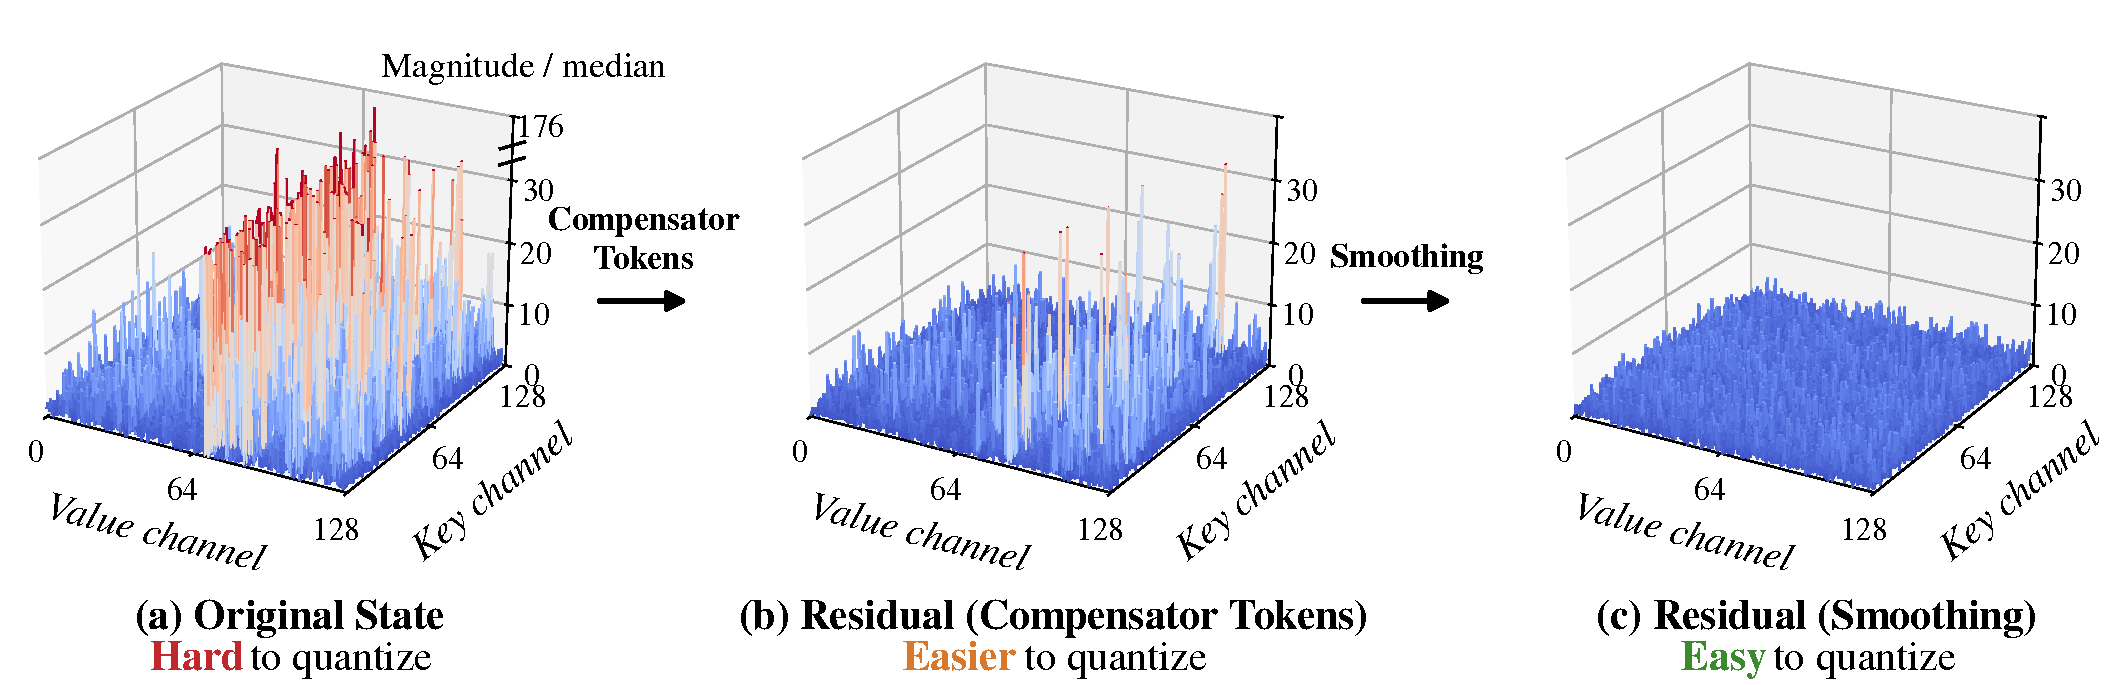
\includegraphics[width=\linewidth]{figures/state_3d.pdf}
        \caption{Magnitude of one Qwen3.5-9B head (layer 13, head 16) at 8K context, normalized by the median magnitude of $S$ in (a) and (b) and of the smoothed residual in (c).
        Outliers up to 176$\times$ the median (a) drop to 47$\times$ after Compensator Tokens (b) and to 5.3$\times$ after smoothing (c).}
        \vspace{-1.5em}
        \label{fig:state-heat}
    \end{minipage}
\end{figure}


The construction extends directly to $r$ compensator tokens.
Let $\tilde K=[\tilde k_1,\ldots,\tilde k_r]\in\mathbb{R}^{d_k\times r}$ and $\tilde U=[\tilde u_1,\ldots,\tilde u_r]\in\mathbb{R}^{d_v\times r}$ collect their vector pairs.
Their combined contribution is
\begin{equation}
  \begin{aligned}
    \tilde K\tilde U^{\top}
       &= \sum_{h=1}^{r}\tilde k_h\tilde u_h^{\top},\\
    R_p &= \hfp{S_p}-\tilde K\tilde U^{\top},
       \qquad \hq{\hat R_p}=\quant_b(R_p),\\
    \hrec{\tilde S_p} &= \dequant_b\bigl(\hq{\hat R_p}\bigr)
       +\tilde K\tilde U^{\top}.
  \end{aligned}
  \label{eq:compensator-rank-r}
\end{equation}
In this way, compensator tokens preserve the dominant state structure in higher precision and leave a residual that is easier to quantize.
For the small values of $r$ used in practice, reconstructing the compensator tokens is fully hidden by the state memory read.
At each window boundary, we refit the compensator tokens on tensor cores without materializing the old ones in the dense state, so for $r\le 8$ the exposed kernel-level overhead stays within 7\% in all settings.

\subsection{Residual smoothing}
\label{sec:round3}

Compensator tokens preserve the dominant low-rank structure in higher precision, but the remaining residual can still have uneven magnitudes across key rows (Figure~\ref{fig:state-heat}(b)).
A few large key- and value-channels can dominate the quantization scale, leaving smaller entries with coarse resolution.
We therefore smooth the residual before quantization to balance its row magnitudes and make it easier to represent at low precision (Figure~\ref{fig:state-heat}(c)).

Let $R_0$ denote the residual at the start of a window.
Each entry of the smoothing vector $c\in\mathbb{R}_{>0}^{d_k}$ is the square root of the corresponding key row's mean absolute value, with a small positive floor to avoid division by zero.
Setting $C=\Diag(c)$, we left-multiply by $C^{-1}$ to balance the key-row magnitudes before quantization.
We quantize this rescaled residual and retain the smoothing scales alongside the quantized residual.
Since the distribution changes over time, these scales remain fixed within each window but are recomputed from the new residual at every boundary.

After dequantization, multiplying by $C$ restores the original key coordinates.
The transform itself is invertible; only the intervening quantization introduces approximation.
Adding back the unchanged higher-precision compensator tokens recovers the initial state.
Substituting this representation into \eqref{eq:window} gives the reconstructed state $S_p$ at the end of the window (Appendix~\ref{app:smoothing} derives the corresponding readout), without changing the buffered real-token updates:
\begin{equation}
  \begin{aligned}
    \hq{\hat R_0^C} &= \quant_b(C^{-1}R_0),\\
    \hfp{S_p} &= \Gamma_{1:p}
      \bigl[C\,\dequant_b\bigl(\hq{\hat R_0^C}\bigr)
          +\tilde K\tilde U^{\top}\bigr]
      +\sum_{j=1}^{p}\Gamma_{j+1:p}\,k_j u_j^{\top}.
  \end{aligned}
  \label{eq:smooth}
\end{equation}
